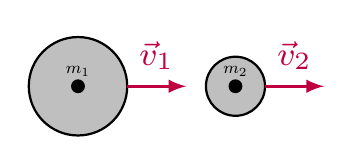
\begin{tikzpicture}
    [
    x=1cm, y=1cm, scale=0.5, font=\footnotesize, >=latex 
    %Voreinstellung für Pfeilspitzen
    ]
    %Raster im Hintergrund
    %\draw[step=1, gray, very thin] (0,0) grid (5.5,5.5);
    
    %m1
    \begin{scope}[xshift=0cm, yshift=0cm, rotate=0, scale=1]
        %Kräfte
        \fill[gray!50!white] (0, 0) circle(1.25);
        \draw[thick] (0, 0) circle(1.25);
        \fill[black] (0, 0) circle(5pt) node [midway, above, yshift=2pt, scale=1.5] {$m_1$};
        \draw [-latex, very thick, purple] (1.25,0) -- ++(1.5,0) node[midway, above, scale=1.5] {$\vec{v}_1$};
    \end{scope}		
    
    %m2
    \begin{scope}[xshift=4cm, yshift=0cm, rotate=0, scale=1]
        %Kräfte
        \fill[gray!50!white] (0, 0) circle(0.75);
        \draw[thick] (0, 0) circle(0.75);
        \fill[black] (0, 0) circle(5pt) node [midway, above, yshift=2pt, scale=1.5] {$m_2$};
        \draw [-latex, very thick, purple] (0.75,0) -- ++(1.5,0) node[midway, above, scale=1.5] {$\vec{v}_2$};
    \end{scope}	
\end{tikzpicture}
